% !TEX root = ../thesis.tex
\chapter{基于自适应相似性矩阵的无监督度量学习}
\section{引言}
数据在数据空间中的空间分布学习一直是一个困难的问题。经验上,数据往往分布在高维空间的一个低维流形上,而不是完全随机分布。这导致了不同标签的数据之间可能有较近的欧氏距离。这种分布特性会对基于传统欧氏距离度量的分类或聚类算法的效果产生影响。一个较好的选择是构建一个能够保持数据对之间局部近邻结构的低维映射。

谱聚类方法是一类在基于矩阵特征分解的聚类方法,该类方法在很多具有挑战性的真实世界数据集上表现出了非常优异的性能。在最近几十年间,一系列经典的谱聚类方法被提出,例如:多维标度法(Multidimensional Scaling,MDS)\cite{cox2000multidimensional},局部线性嵌入(Local Linear Embedding,LLE)\cite{roweis2000nonlinear},等距特征映射(Isomap)\cite{tenenbaum2000global},拉普拉斯特征映射(Laplacian Eigenmaps)  \cite{belkin2001laplacian}和变种的谱聚类\cite{ng2002spectral}. 上述提到的谱聚类算法有三点不足之处。第一,这些谱聚类算法只提供了训练数据的嵌入映射,对样本外数据(out-of-sample)的计算比较困难。第二,这些算法的复杂度依赖于数据点数量,相对比较耗时,可扩展性不强。第三,谱聚类算法的稳定性高度依赖于相似性图(affinity graph)的鲁棒性。

为缓解上述谱聚类中存在的问题,大量重要的研究进展被提出\cite{bengio2004out,niyogi2004locality,fowlkes2004spectral,yan2009fast,chen2011large,pavan2007dominant,premachandran2013consensus,zhu2014constructing,nie2014clustering}。局部保持投影(Locality Preserving Projections, LPP)\cite{niyogi2004locality}引入了一种由拉普拉斯特征映射得到的线性投影方法。他们的工作提供了一种嵌入映射的线性近似,该线性近似可以减少计算复杂度并可以简单的实现样本外数据的扩展。线性嵌入提供了一种度量学习角度下的谱聚类方法。文献\parencite{nie2014clustering}提出了自适应近邻投影聚类(Projected Clustering with Adaptive Neighbors,PCAN)算法,该算法将点对之间的相似性作为一个额外的待求解变量并且通过对图拉普拉斯(graph Laplacian)矩阵的秩设置惩罚项以限制相似性矩阵的连通区数量。基于这个框架,PCAN算法交替地更新相似性矩阵和投影。

\begin{figure}[!hbtp]
	%\centering
	\subfigure[Ideal affinity matrix]{
			\begin{minipage}[t]{0.14\textwidth}
				\centering
				
\includegraphics[width=1\columnwidth]{k1.jpg}
			\end{minipage}
		}
		\subfigure[Heat kernel with $k=100$]{
			\begin{minipage}[t]{0.14\textwidth}
				\centering
				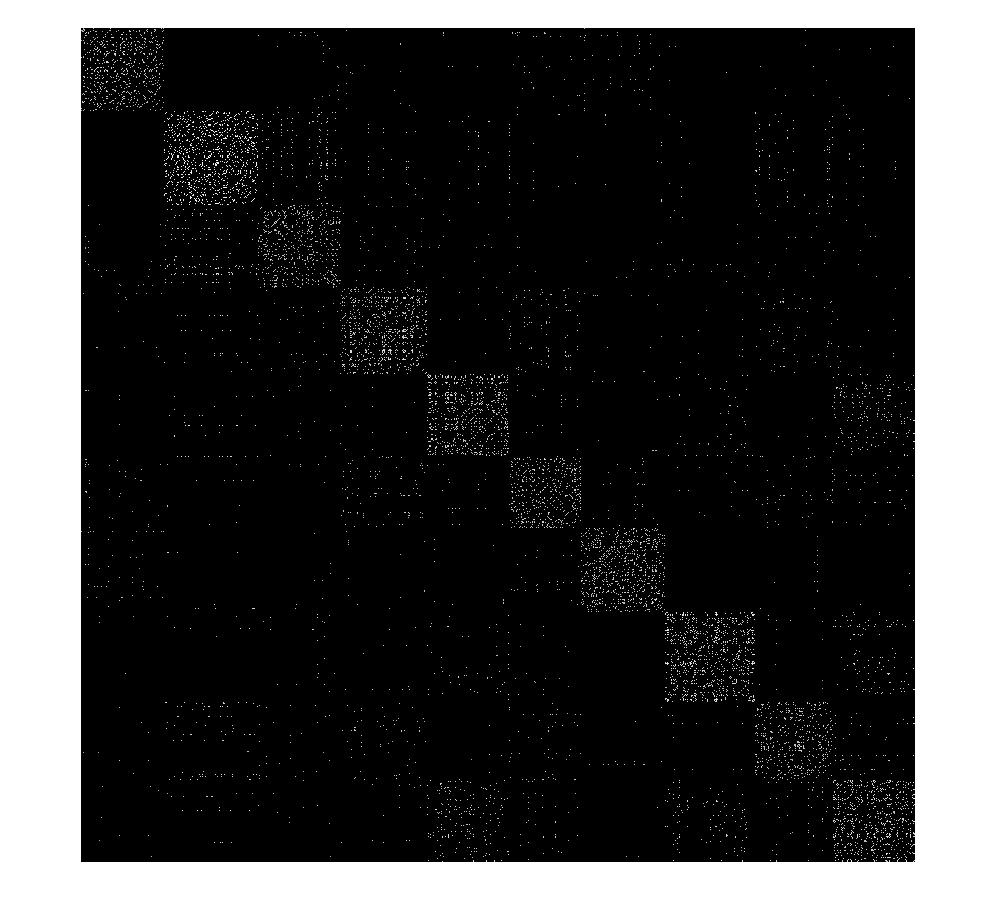
\includegraphics[width=1\columnwidth]{k100.jpg}
			\end{minipage}
		}
		\subfigure[Heat kernel with $k=1000$]{
			\begin{minipage}[t]{0.14\textwidth}
				\centering
				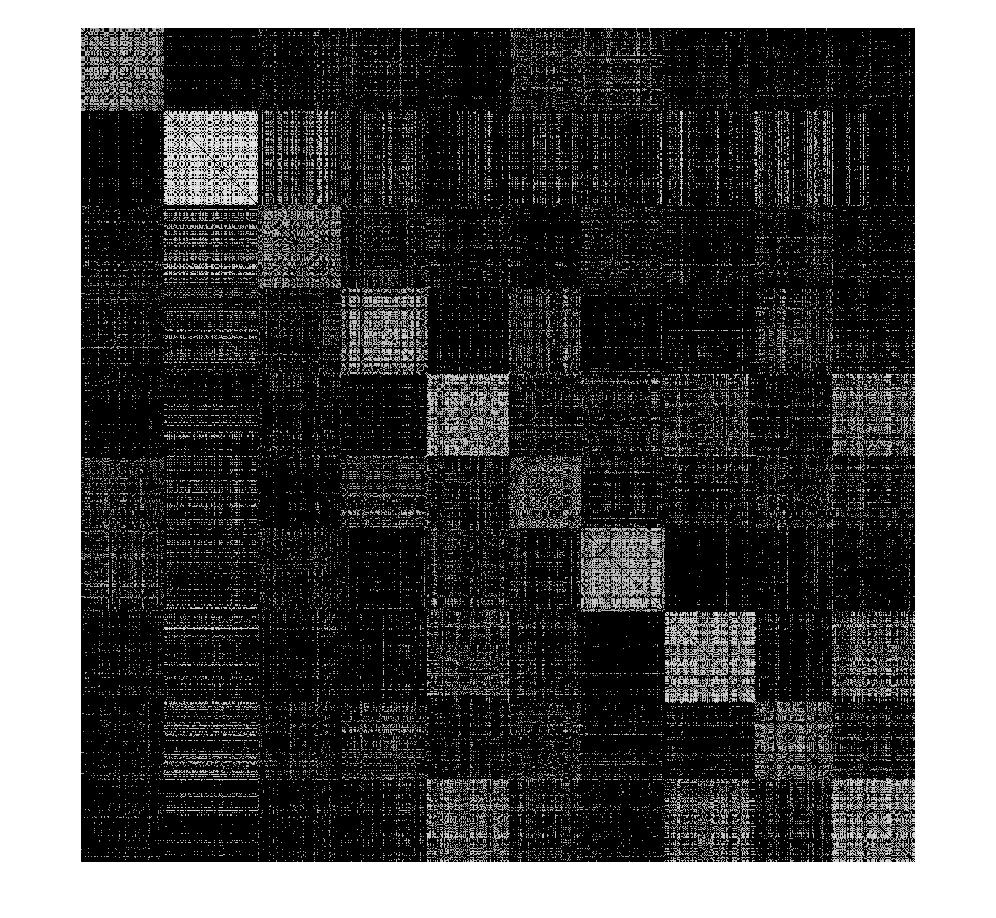
\includegraphics[width=1\columnwidth]{k1000.jpg}
			\end{minipage}
		}
	
	
	\caption{Affinity matrices of a subset of MNIST}
	\label{affMat1}
\end{figure} 


\begin{figure}[!hbtp]
  \centering
  \bisubcaptionbox{$R_3 = 1.5\text{mm}$ 时轴承的压力分布云图}%
                  {Pressure contour of bearing when $R_3 = 1.5\text{mm}$}%
                  [6.4cm]{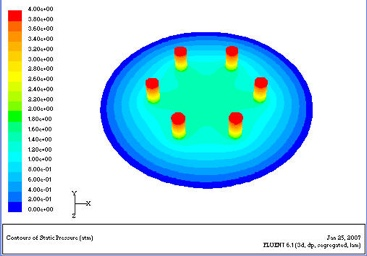
\includegraphics[height=2.5cm]{pressure15.jpg}}
  \hspace{1cm}
  \bisubcaptionbox{$R_3 = 2.5\text{mm}$ 时轴承的压力分布云图}%
                  {Pressure contour of bearing when $R_3 = 2.5\text{mm}$}%
                  [6.4cm]{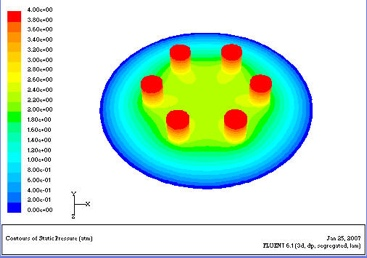
\includegraphics[height=2.5cm]{/pressure25.jpg}}
  \bicaption{包含子图题的范例(使用 subcaptionbox)}
            {Example with subcaptionbox}
  \label{fig:bisubcaptionbox}
\end{figure}